\chapter{$^{3}$He Polarimetry}
\label{chap:chap3}

\section{Overview}

Traditional pure glass target cells are studied mainly using Adiabatic Fast Passage (AFP) Nuclear Magnetic Resonance (NMR) and Electron Paramagnetic Resonance (EPR). AFP is a technique that allows us to monitor a signal that's directly proportional to the ${3}He$ polarization, which then provides a means to gain knowledge of properties of cell including pumping time and relaxation rates. The EPR technique utilizes the fact that polarized $^{3}$He produces frequency shift of the magnetic resonance lines of alkali metal to measure the $^{3}$He polarization. When AFP and EPR are combined, we can calculate the calibration constant between AFP signal and $^{3}$He polarization. 

A significant focus of my studies is on exploring cells that incorporate metal. Unfortunately, AFP is not suitable for studying these cells as it requires exposing the entirety of the cell to a Radio Frequency magnetic field in an attempt to flip all spins in the cell. For these cells, Pulsed Nuclear Magnetic Resonance (PNMR) has proven to be very useful. PNMR only applies a pulsed RF field to a small selected part of the cell which makes it relatively easy to prevent metal from distorting the signal. However, the spins tipped by applying the pulse lose their transverse component (which depends on the "tip angle"), we typically allow some time for this portion of gas to diffuse out of the region before taking the next measurement on a fresh sample of the gas. The rate at which measurements are taken is limited by this requirement.

This chapter introduces the three techniques mentioned above and how they're used for our studies.

\section{Adiabatic Fast Passage}

\subsection{Nuclear Magnetic Resonance}

The energy of a magnetic moment in an external field is

\begin{equation}
E = -\vec{\mu}\cdot \vec{B_{0}} = -\mu_{z}B_{0}
\end{equation}

where $\vec{\mu}$ is the magnetic moment, for a spin-1/2 nuclei, the energy is

\begin{equation}
E = -\gamma B_{0}\hbar/2
\end{equation}

$\gamma$ is the gyromagnetic ratio, $\gamma /2\pi \approx 3.2434kHz/Gauss$. When a oscillating magnetic field with the frequency $\omega=\gamma B_{0}$ is present, transitions between the +1/2 and -1/2 states are induced. This frequency is called Larmor frequency. When a nucleus is placed in an external magnetic field that is not aligned with its magnetic moment, it will precess at the Larmor frequency.

\subsection{The Rotating Coordinate System}

\subsubsection{Classical Formulation}

For a nucleus in an external field $\vec{B}$ with $\gamma \hbar \vec{I}$ as its nuclear angular momentum, the equation of motion in a stationary coordinate system is \cite{RevModPhys.26.167}

\begin{equation}\label{eq1}
\hbar \frac{d\vec{I}}{dt}=\gamma \hbar \vec{I} \times \vec{B}
\end{equation}

Let $\frac{\partial}{\partial t}$ represent the derivative with respect to a coordinate system that rotates with angular velocity $\vec{\omega}$,

\begin{equation}{eq2}
\frac{d\vec{I}}{dt}=\frac{\partial \vec{I}}{\partial t}+\vec{\omega} \times \vec{I}
\end{equation}

Substitute Eq.\@ \ref{eq2} into Eq.\@ \ref{eq1}, $\vec{I}$ in the rotating frame satisfies the equation of motion 

\begin{equation}
\hbar \frac{\partial \vec{I}}{\partial t}=\gamma \hbar \vec{I} \times (\vec{B} + \vec{\omega}/\gamma)=\gamma \hbar \vec{I} \times \vec{B_{eff}}
\end{equation}

where $\vec{B_{eff}}$ is the effective field in the rotating frame

\begin{equation}
\vec{B_{eff}}=\vec{B} + \vec{\omega}/\gamma
\end{equation}

Thus, for an observer in the rotating frame, the net effect is the same as changing the field to include an additional term $\omega/\gamma$.

If we apply this result to rotating magnetic fields, we will get the core idea of performing an Adiabatic Fast Passage (AFP) measurement. Assuming a constant field $\vec{B}$ and another field $\vec{B_{1}}$ perpendicular to $\vec{B}$ and rotates with angular velocity $-\omega$. In the rotating frame that rotates with $\vec{B_{1}}$, both aforementioned field are constant. The effective field in the rotating frame is

\begin{equation}\label{EffectiveField}
B_{eff}\vec{z}=(B-\omega/\gamma)\vec{z} + B_{1}\vec{x'}
\end{equation}

where $\vec{x'}$ is the direction that $\vec{B_{1}}$ is in. When on resonance (B = $\omega/\gamma$), the effective field is perpendicular to the constant field $\vec{B}$.

\subsubsection{Quantum Mechanical Formulation}

The Shr$\ddot{o}$dinger equation for a magnetic moment in an external field is

\begin{equation}\label{eq3}
i\hbar \dot{\psi}=\mathcal{H} \psi=-\gamma \hbar \vec{I}\cdot \vec{B} \psi
\end{equation}

Let $\psi$ and $\vec{B}$ be the wave function and magnetic field in a stationary frame and $\psi_{r}$ and $\vec{B_{r}}$ be the same quantities in a rotating frame with angular velocity $\vec{\omega}$. Using the rotation operator in quantum mechanics, 

\begin{subequations}\label{eq4}
	\begin{gather}
	\psi=e^{-i\vec{\omega}\cdot \vec{I}t}\psi_{r} \\
	\vec{I}\cdot \vec{B_{r}} = e^{i\vec{\omega}\cdot \vec{I}t}\vec{I}\cdot \vec{B} e^{-i\vec{\omega}\cdot \vec{I}t}
	\end{gather}
\end{subequations}

Substituting \ref{eq3} into Eq.\ref{eq3}, the Shr$\ddot{o}$dinger equation in the rotating frame is obtained

\begin{equation}
i\hbar \dot{\psi_{r}}=-\gamma \hbar \vec{I}\cdot(\vec{B_{r}} + \vec{\omega}/\gamma)\psi_{r}=-\gamma \hbar \vec{I}\cdot\vec{B_{eff}}\psi_{r}
\end{equation}

The same effective field in the rotating frame is reached as that from the classical derivation.

\subsection{Adiabatic Fast Passage}

Adiabatic Fast Passage (AFP) NMR is used to measure the $^{e}$He polarization. In an AFP measurement, with the assistance of a oscillating radiofrequency (RF) field, the spins follow the effective field in a rotating frame (as discussed in more detail below) and are flipped 180 degrees to the opposite direction and then flipped back, producing two peaks in signal when they're perpendicular to the pick up coils.

The flipping process can be achieved by either sweeping the main holding field or sweeping the RF frequency so that the longitudinal component of effective field in the rotating field goes through zero. AFP measurements in out lab are typically done by sweeping the holding field while keeping the RF frequency constant. The RF coils produce a RF field of magnitude 2$B_{1}$ perpendicular to the main holding field B. The oscillating field has a frequency of $\omega$ and can be decomposed into two counter-rotating components with the same amplitude B$_{1}$. Only the component rotating in direction to be able to give a resonance in Eq.\ref{EffectiveField} has an important effect. In this frame, the effective field is

\begin{equation}
B_{eff}\vec{z}=(B-\omega/\gamma)\vec{z} + B_{1}\vec{x'}
\end{equation}

as discussed above. The other rotating component does not affect the spins. In an AFP measurement, the holding field starts from a value that's lower than $\omega/\gamma$ ($\omega/\gamma-B\gg B_{1}$), so that the effective field is almost aligned with the holding field (and the spins). The holding field is then swept at a constant rate through resonance to a value greater than $\omega/\gamma$. The sweeping rate is of great importance. The sweep needs to be slow enough so that the nuclear spins can follow the effective field

\begin{equation}
\frac{\dot B}{B_{1}}\ll \omega
\end{equation}

Sweep that satisfies this condition is considered as adiabatic.

Sweep rate cannot be too slow either, because the relaxation rate of the spins are faster near the resonance especially with a small effective field. The relaxation rate of $^{3}$He in the rotating frame at resonance is 

\begin{equation}
\frac{1}{T_{1r}}=D\frac{|\nabla B_{z}|^{2}}{B_{1}^{2}} 
\end{equation}

where D is the $^{3}$He diffusion constant. In order to keep the AFP loss low, it's important for the time scale that the spins stay close to resonance to be much shorter than $1/T_{1r}$:

\begin{equation}
D\frac{|\nabla B_{z}|^{2}}{B_{1}^{2}} \ll \frac{\dot B}{B_{1}}
\end{equation}

Typically, the field is swept from 12.6 Gauss to 20.4 Gauss in 6s, thus

\begin{subequations}
	\begin{gather}
	\dot B = 1.3G/s\\
	B1 \approx 100mG\\
	f = 56.6kHz\\
	D \approx 0.16cm^2/s\\
	|\nabla B_{z}| \approx 10mG/cm\\
	\end{gather}
\end{subequations}

With these operating conditions, 

\begin{subequations}
	\begin{gather}
	D\frac{|\nabla B_{z}|^{2}}{B_{1}^{2}} \approx 1.6mHz\\
	frac{\dot B}{B_{1}} \approx 13Hz\\
	w \approx 356kHz
	\end{gather}
\end{subequations}

The AFP conditions are clearly well satisfied. Fig.\ref{AFP} shows the evolution of effective field during an AFP measurement.

\begin{figure}[H]
	\centering
	\resizebox{0.91\textwidth}{!}{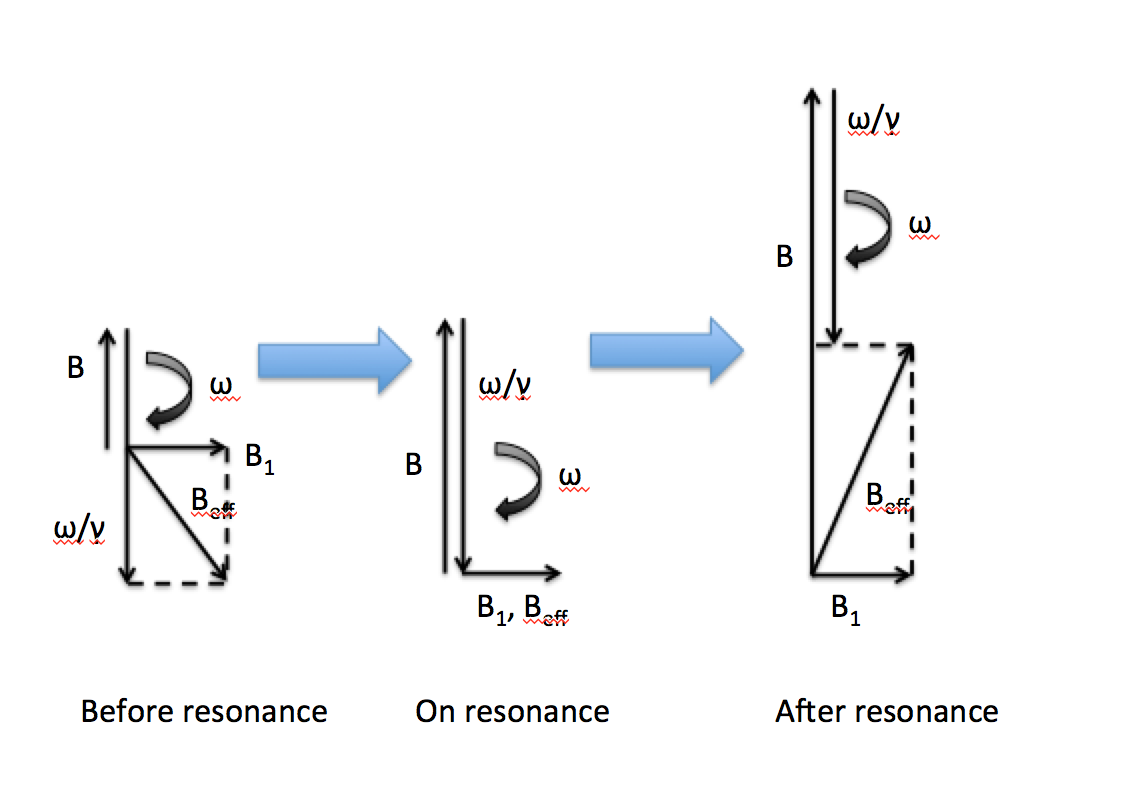
\includegraphics{AFP.png}}
	\caption{{\bf Effective field in the rotating frame during an Adiabatic Fast Passage measurement. The $^{3}He$ spins follow the direction of the effective field. $B_{1}$ is exaggerated to show different components of effective field clearly.}}
	\label{AFP}
\end{figure}

The pick up coils are placed close to the cell and perpendicular to the holding field and RF field. As the $^{3}$He spins precess along the holding field, the transverse component of the spins will induce an electromotive force (EMF) that is directly proportional to the amplitude of the component in the pick up coils. The signal can be written as:

\begin{equation}
S=A\omega \sin{\alpha(t)}=A\omega \frac{B_{1}}{B_{1}^{2}+(B(t)-\omega/\gamma)^{2}}
\end{equation}

where A is a constant that accounts for the cell and coils geometry, the cell magnetization and the electronics factors that affect the size of signal; $\omega$ is the RF frequency; $\alpha$ is the angle between the effective field and the holding field in the rotating frame; B(t) is the holding field as a function of time. The signal reaches peak value when B(t) = $\omega/\gamma$. Fig.\ref{AFPSignal} shows the result of a typical AFP measurement.

\begin{figure}[H]\label{AFPSignal}
	\centering
	\resizebox{0.91\textwidth}{!}{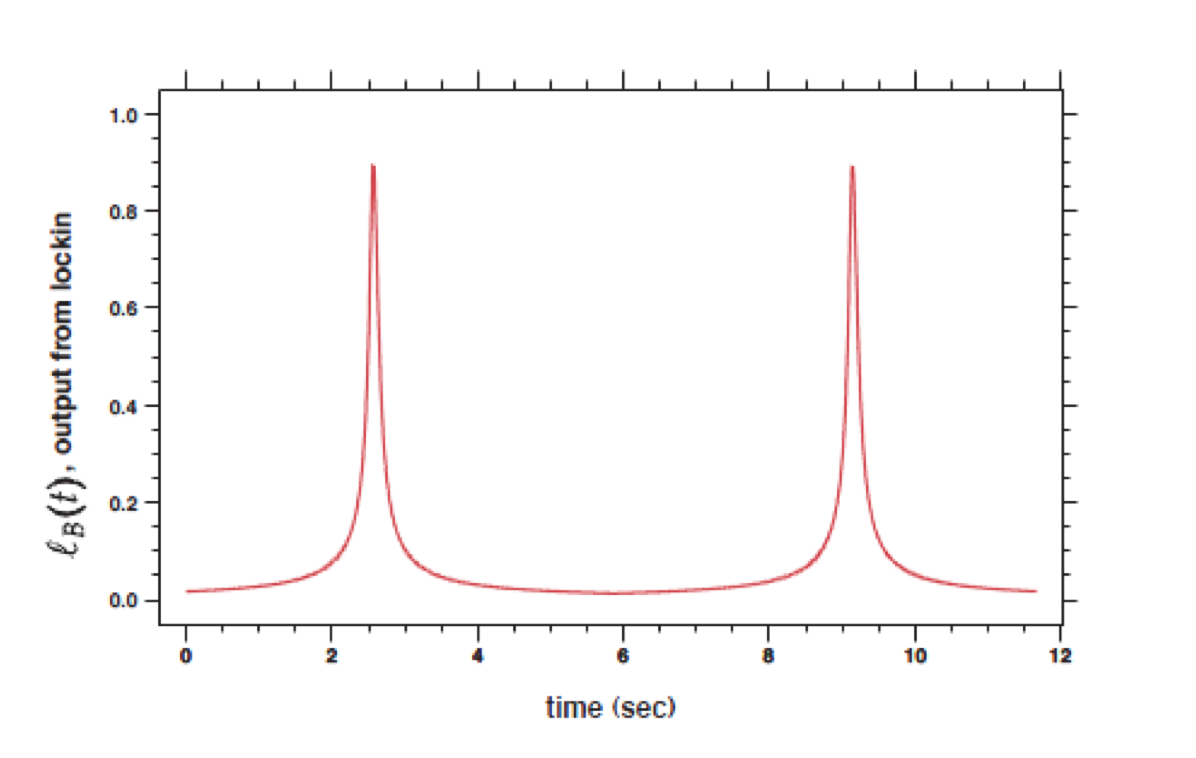
\includegraphics{AFPSignal.png}}
	\caption{{\bf A typical AFP signal. y axis is in arbitrary unit.}}
	\label{AFPSignal}
\end{figure}

\subsection{Spinups and Spindowns}

As previously mentioned, AFP is used to monitor the polarization of $^{3}$He. An exact value of polarization remains to be calibrated with EPR, but the signal size is directly proportional to the polarization, thus is an indication of how the polarization changes relatively. Two processes that are monitored with AFP are spinups and spindowns. 

\subsubsection{Double-Chambered Cell Spinup}

The process of $^{3}$He gaining polarization through spin-exchange with Rb that are being constantly pumped by circularly polarized laser is called spinup. The equation that describes spinups of single-chambered cell was already discussed in Chapter 2. But target cells used in electron-scattering experiments are normally composed of two chambers: a pumping chamber (PC), which is placed in an oven and pumped by circularly polarized laser, and a target chamber (TC) that the electron beam passes through. Fig.\ref{TargetCell} shows a typical cell.

\begin{figure}[H]
	\centering
	\resizebox{0.91\textwidth}{!}{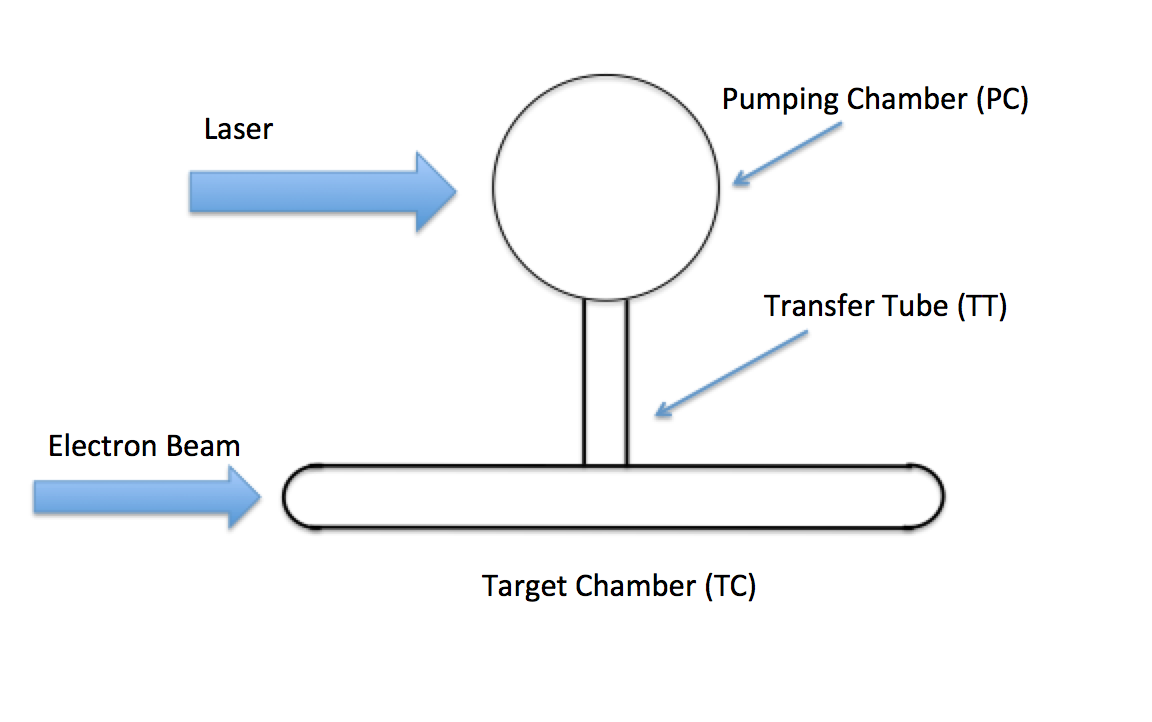
\includegraphics{TargetCell.png}}
	\caption{{\bf A target cell. The dimensions of different parts of the cell is not to scale.}}
	\label{TargetCell}
\end{figure}

As only the $^{3}$He nuclei in the pumping chamber are gaining polarization and the electron beam constantly causes additional relaxation in the target chamber, it is important that the $^{3}$He from PC can replenish the polarization in TC quickly enough. Before the 12GeV upgrade of JLab, this was normally achieved through diffusion. With higher electron beam after the upgrade, it is currently planned the design of the cell will be changed. The number of transfer tubes will be increased to two with one of them being heated causing a temperature gradient between the two transfer tubes and driving controllable convection. This new design is called convection cell and is discussed thoroughly by Dolph\ref{PhysRevC.84.065201}. The following derivation will only focus on the old design with diffusion for simplicity. The polarization accumulation process can be described by 

\begin{subequations}\label{DoubleChamber}
	\begin{gather}
	\frac{dP_{PC}}{dt}=\gamma_{se}(P_{A}-P_{PC})-\Gamma_{PC}P_{PC}-d_{PC}(P_{PC}-P_{TC})\\
	\frac{dP_{TC}}{dt}=-\Gamma_{TC}P_{TC}+d_{TC}(P_{PC}-P_{TC})
	\end{gather}
\end{subequations}

where $P_{PC} (P_{TC})$ is the $^{3}$He polarization in PC (TC); $\gamma_{se}$ is the spin-exchange rate in PC; $\Gamma_{PC} (\Gamma_{TC})$  is the relaxation rate o $^{3}$He polarization in PC (TC); $d_{PC} (d_{TC})$ is the probability for a nucleus to leave PC (TC) and enter TC (PC). The transfer rates $d_{PC}$ and $d_{TC}$ are related by:

\begin{equation}
f_{PC}d_{PC}=f_{TC}d_{TC}
\end{equation}

where $f_{PC} (f_{TC})$ is the fraction of atoms in PC (TC). The solutions to Eq.\ref{DoubleChamber} are

\begin{subequations}\label{DoubleChamberSolution}
	\begin{gather}
	P_{PC}(t)=C_{PC}e^{-\gamma_{f}t}+(P_{PC}^{0}-P_{PC}^{\infty}-C_{PC})e^{-\gamma_{s}t}+P_{PC}^{\infty}\\
	P_{TC}(t)=C_{TC}e^{-\gamma_{f}t}+(P_{TC}^{0}-P_{TC}^{\infty}-C_{TC})e^{-\gamma_{s}t}+P_{TC}^{\infty}
	\end{gather}
\end{subequations}

Detailed discussion is done by Dolph\ref{PhysRevC.84.065201}. It's interesting to note the time evolution of $^{3}$He polarization for double-chambered cells has two time constant: the fast time constant $\gamma_{f}$ that is dominated by the diffusion rates $d_{PC}$ and $d_{TC}$ when diffusion is relatively fast, and the slow time constant $\gamma_{S}$ that is mostly determined by the volume averaged spin-exchange rate. In the fast-transfer limit, double-chambered solution reduces to single-chambered solution. 

The other interesting point is the relation between the saturation polarization in PC and TC:

\begin{equation}
P_{TC}^{\infty}=\frac{P_{PC}^{\infty}}{1+\frac{\Gamma_{TC}}{d_{TC}}}
\end{equation}

Again, in the fast-transfer limit where $d_{TC}\gg \Gamma_{TC}$, $P_{TC}^{\infty}=P_{PC}^{\infty}$. Fig.\ref{BradySpinup} shows the spinup curves for a double-chambered cell. This spinup is different than regular ones in that the AFP measurements were taken every 3 minutes (normal sample rate is one AFP every one hour), thus the losses due to frequent measurements limited the saturation polarization. The raw signal obtained from AFP have already been calibrated by EPR so the y axis is polarization rather than raw signal amplitude. 

\begin{figure}[H]
	\centering
	\resizebox{0.91\textwidth}{!}{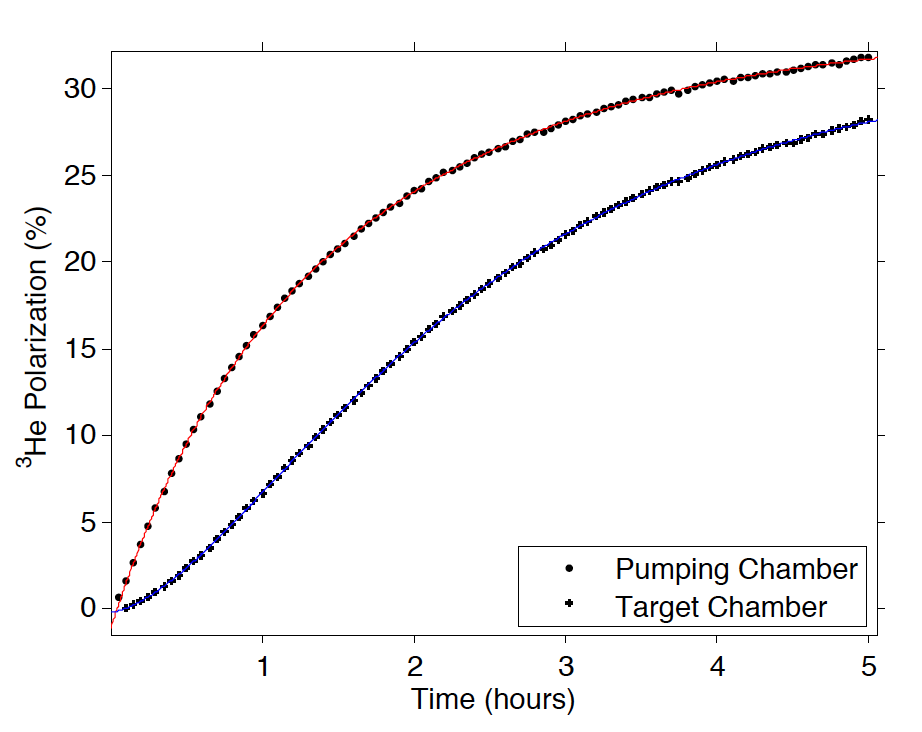
\includegraphics{BradySpinup.png}}
	\caption{{\bf $^{3}$He polarization as a function of time for both the pumping chamber and the target chamber. The top curve is the pumping chamber and the bottom curve is the target chamber.}}
	\label{BradySpinup}
\end{figure}

\subsubsection{Initial Spinup}

As shown in Fig.\ref{BradySpinup}, the early spinup behaviors of the pumping chamber and the target chamber are quite different. The initial part of the pumping chamber is almost linear but the target chamber shows a curved initial part. By performing a Taylor expansion on Eq.\ref{DoubleChamberSolution} we obtain the initial part of the spinup for both chambers:

\begin{subequations}\label{InitialSpinup}
	\begin{gather}
	P_{PC}(t)=\gamma_{se}P_{A}t-\frac{1}{2}\gamma_{se}P_{A}(\gamma_{se}+\Gamma_{PC}+d_{PC})t^{2}\\
	P_{TC}(t)=\frac{1}{2}\gamma_{se}P_{A}d_{TC}t^{2}
	\end{gather}
\end{subequations}

where $\gamma_{se}$ is the spin-exchange rate in the pumping chamber and $P_{A}$ is the alkali polarization. It's clear that the dominant term in $P_{PC}(t)$ is the linear term while the shape of $P_{TC}(t)$ is quadratic. 

The slope of the linear shape of initial spinup of the pumping chamber gives access to the product $P_{A}\gamma_{se}$ and fitting the initial spinup of the target chamber to a quadratic function provides the product $\gamma_{se}P_{A}d_{TC}$. The alkali polarization $P_{A}$ can be measured with the technique named Faraday Rotation, we then gain knowledge of the spin-exchange rate $\gamma_{se}$ and the diffusion rate $d_{TC}$.

\subsubsection{Spindown}

The spin relaxation rates in the pumping chamber and the target chamber are different due to geometry and other properties. The cell-average relaxation rate can then be written as

\begin{equation}
\langle \Gamma \rangle=f_{PC}\Gamma_{PC}+f_{TC}\Gamma_{TC}
\end{equation}

where $f_{PC}$ ($f_{TC}$) is the fraction of atoms in PC (TC); $\Gamma_{PC}$ ($\Gamma_{TC}$) is the average relaxation rate in PC (TC). When the cell is being pumped by laser, the pumping chamber is heated with hot air to create alkali vapor while the target chamber remains at the room temperature. The difference in temperature adds to the difference in relaxation rates. However, when trying to measure the life time (the inverse of the relaxation rate) of the cell, we typically keep the entire cell at room temperature and perform a "spindown" measurement. 

During a spindown, the cell starts with some polarization (normally as high as possible so we can obtain a more complete curve), and relaxes on its own while we take AFP measurements at a certain rate. Typically, the interval between measurements is anywhere between 30 mins and 2 hrs, depending on the lifetime of the cell. The rule of thumb is to take AFP frequently enough so the spindown curve has sufficient data points while not too often so the polarization relaxes much faster due to AFP losses. The $^{3}$He polarization relaxation can be described by

\begin{equation}\label{Spindown}
P(t)=P_{0}e^{-t/\tau_{true}}
\end{equation}

The true lifetime $\tau_{true}$ of the cell without relaxation due to AFP loss can be measured with two methods: the first is to take 5 AFP measurements consecutively with very short interval (normally around 3 minutes), the second is to perform several spindown measurements, each with a different interval. 

In the first method, because the lifetime of the cell is much longer than 3 minutes, we can safely attribute all losses to AFP measurements and extract the loss due to a single AFP $loss_{afp}$. The data values can then be corrected with the equation

\begin{equation}
S_{i}^{corrected}=S_{i}^{raw}/(1-loss_{afp})^{i}
\end{equation}

where $S_{i}^{corrected}$ is the corrected signal, $S_{i}^{raw}$ is the raw signal, i represents it is the $i$th measurement in the spindown, $loss_{afp}$ is the loss due to a single measurement. Fitting the corrected values to Eq.\ref{Spindown} gives the true lifetime $\tau_{true}$.

A simple example for the second method would be to perform one spindown with one-hour interval and another spindown with two-hour interval, the relaxation rates in these two spindowns are

\begin{subequations}
	\begin{equation}
	\frac{1}{\tau_{1hr}}=\frac{1}{\tau_{true}}+\Gamma_{AFP\_1hr}
	\end{equation}
	\begin{equation}
	\frac{1}{\tau_{2hr}}=\frac{1}{\tau_{true}}+\Gamma_{AFP\_2hr}
	\end{equation}
	\begin{equation}
	\Gamma_{AFP\_1hr}=2\times \Gamma_{AFP\_2hr}
	\end{equation}
\end{subequations}

where $\tau_{1hr}$ and $\tau_{2hr}$ are the lifetimes measured with taking AFP every 1 hour and every 2 hours, $\tau_{true}$ is the true lifetime of the cell without interference from measurements, $\Gamma_{AFP\_1hr}$ ($\Gamma_{AFP\_2hr}$)is the relaxation rate due to taking measurements every 1hr (2hr). We can then solve for $\tau_{true}$.

\subsection{AFP Loss}

The longitudinal spin relaxation rate due to static field inhomogeneities is

\begin{equation}
\frac{1}{T_{1}} = D\frac{|\nabla B_{x}|^{2}+|\nabla B_{y}|^{2}}{B_{0}^{2}}
\end{equation}

where D is the diffusion constant for the polarized spins, and is inversely proportional to the gas pressure. $B_{0}$ is the mean magnetic field along z axis. $B_{x}$ and $B_{y}$ are the x and y components of the magnetic field. However, when performing AFP measurement, the spins are exposed to a small oscillating RF field, the spin relaxation can be greatly accelerated under magnetic resonance conditions~\cite{PhysRevA.38.5092},

\begin{equation}
\frac{1}{T_{r1}} = \frac{8R^{4}}{175D}|\nabla \Omega_{z}|^{2}\sum_{n} \frac{175}{4(\chi_{1n}^{2}-2)(\chi_{1n}^{4}+r^{2}+r^{2}s^{2})(1+s^{2})}
\end{equation}

where R is the cell radius, D is the diffusion constant, $\Omega_{z}$ is the Larmor frequency of the holding field, $r=\frac{\omega_{r}R^{2}}{D}$, $s=\frac{\Omega_{0}-\omega}{\omega_{r}}$, the numbers $\chi_{1n}$ are the zeros of the derivatives of the spherical Bessel functions

\begin{equation}
\frac{d}{dx}j_{1}(x_{1n})=0~for~n=1,2,3...
\end{equation}

Since $r^{2}\gg \chi_{1n}^{4}$, and $\sum_{n}\frac{1}{\chi_{1n}^{2}-2}=\frac{1}{2}$~\cite{PhysRevA.37.2877},

\begin{equation}
\frac{1}{T_{r1}}=\frac{R^{4}|\nabla\Omega_{z}|^{2}}{r^{2}(1+s^{2})^{2}D}=\frac{|\nabla B_{z}|^{2}D}{B^{2}(1+s^{2})^2}
\end{equation}

If $P_{0}$ the is the polarization before AFP, the polarization P after a single AFP flip is given by 

\begin{equation}
P=P_{0}e^{-\int \Gamma_{r1} dt}=P_{0}e^{-\int \frac{1}{T_{r1}}dt}
\end{equation}

Given the field sweep starts from 12.6G, ends at 20.4G, the RF frequency is 56.6kHZ, the sweep time is 6s and $B_{1}$ is 100mG, we can safely approximate the integral by 

\begin{equation}
\int_{-\infty}^{\infty} \frac{1}{T_{r1}}dt=\frac{\pi D|\nabla B_{z}|^{2}}{2B_{1}\partial B_{1}/\partial t}
\end{equation}

which is the fractional loss due to a single AFP flip.

To better understand AFP loss, we did a study where we took AFP measurements at various different field gradients to study the relation between AFP loss and inhomogeneities. The gradients were produced by Maxwell-style transverse gradient coils and increased from 0 to a little under 160 mG/cm. At each set gradient, we take one AFP to look at the difference between the two peaks to determine the loss due to a single flip. Fig~\ref{AFPLossvsGradient} shows AFP losses collected from experiments and theoretical predictions. They agree mostly within the error bar.

\begin{figure}[H]
	\centering
	\resizebox{0.91\textwidth}{!}{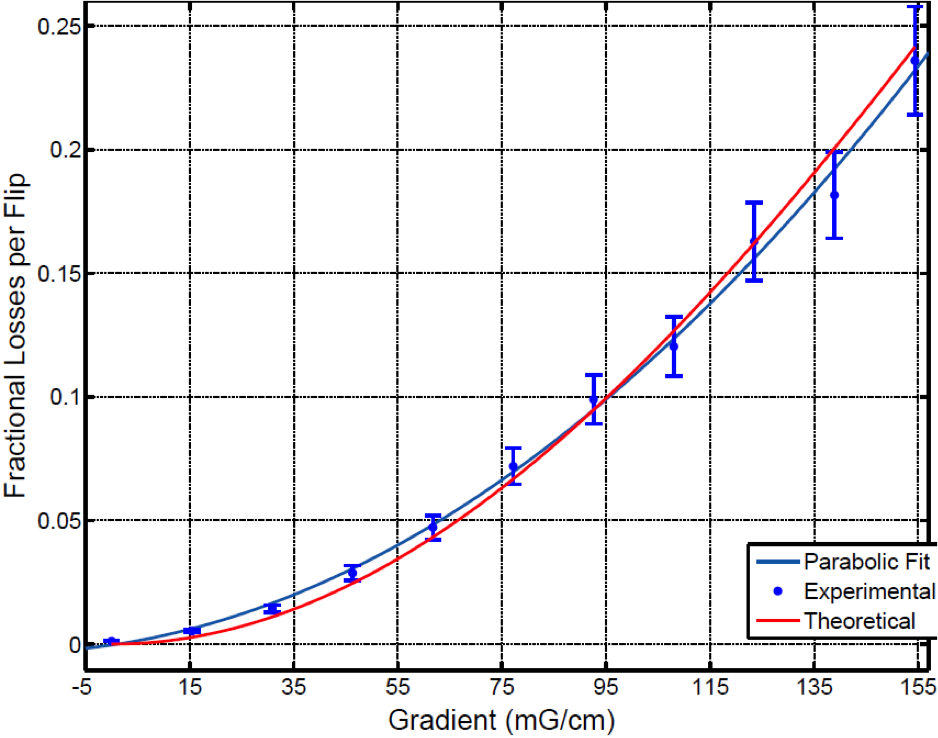
\includegraphics{AFPLossvsGradient.png}}
	\caption{{\bf Fractional AFP loss (single flip) as a function of field gradient.}}
	\label{AFPLossvsGradient}
\end{figure}

\section{Electron Paramagnetic Resonance}

\subsection{Overview}

Electron Paramagnetic Resonance (EPR) is a important technique for measuring the frequency shift of alkali metal Zeeman resonance due to the effective magnetic field produced by polarized $^{3}He$ gas. The EPR shift is largely caused by the Fermi-contact interaction $\alpha$ {\bf K$\cdot$S} between the nuclear spin {\bf K} of the noble gas nucleus of magnetic moment $\mu_{K}$ and the electron spin {\bf S} of the alkali metal atom~\cite{PhysRevA.71.013414}. The magnetic field created by the bulk magnetization of the $^{3}He$ gas also contributes directly to a relatively small part of the shift (rougly 1/6 for K). The total measured shift is therefore written as the expected Zeeman interaction with the field produced by the polarized $^{3}He$ multiplied by an enhancement factor $\kappa_{0}$. The enhancement effect comes from overlapping of alkali metal electrons and $^{3}$He nucleus during binary collisions, thus $\kappa_{0}$ is different for each alkali metal species and slightly temperature dependent.

During the process of optical pumping, the Rb atoms are excited to the 5P$_{\frac{1}{2}}$ state by the pump laser. The majority of these atoms are quenched non-radiatively to the ground state by N$_{2}$. While at 5P$_{\frac{1}{2}}$ state, Rb atoms can also be excited to the 5P$_{\frac{3}{2}}$ state through collisions with other Rb atoms. A small fraction of the excited atoms (5P$_{\frac{1}{2}}$ and 5P$_{\frac{3}{2}}$) decay by emitting either a D$_{1}$ photon or D$_{2}$ photon. The intensity of fluorescence is proportional to the excited Rb atoms, thus is higher when the Rb polarization is low so more Rb atoms can absorb laser and be excited. We typically induce Zeeman transitions with a RF coil to lower alkali polarization and detect D$_{2}$ photons with a photodiode behind a D$_{2}$ filter. The highest amount of D$_{2}$ photons is detected when the RF frequency is exactly equal to the Zeeman transition frequency.

\subsection{The Breit-Rabi Equation}

The Zeeman energy levels of ground state (L = 0) can be described with the Breit-Rabi equation

\begin{equation}
E_{F=I\pm 1/2, m_{F}}=-\frac{h\Delta \nu_{hfs}}{2(2I+1)}-\mu_{N}g_{I}Bm_{F}\pm \frac{h\Delta \nu_{hfs}}{2}\sqrt{1+\frac{4m_{F}x}{2I+1} +x^{2}}
\end{equation}

where

\begin{equation}
x=(g_{I}\mu_{N}-g_{s}\mu_{B})\frac{B}{h\Delta \nu_{hfs}}
\end{equation}

B is the magnetic field, $\Delta \nu_{hfs}$ is the hyperfine splitting frequency, I is the nuclear spin, $g_{I}$ and $g_{s}$ are the g factors of nuclear and electron spin, $\mu_{N}$ and $\mu_{B}$ are the nuclear and Bohr magneton, respectively. 

The Zeeman transition frequency of $m_{F} \rightarrow m_{F} - 1$ is 

\begin{equation}
\begin{split}
\nu_{m_{F}\rightarrow m_{F-1}} &=\frac{E_{F,m_{F}}-E_{F,m_{F}-1}}{h} \\
&= -\frac{g_{I}\mu_{N}B}{h}\pm \frac{\Delta \nu_{hfs}}{2}\left(\sqrt{1+\frac{4m_{F}}{2I+1}x+x^{2}}-\sqrt{1+\frac{4m_{F}-1}{2I+1}x+x^{2}}\right)
\end{split}
\end{equation}

The second term is much greater than the first term under our operating conditions, so the sign of the frequency $\nu_{m_{F}\rightarrow m_{F-1}}$ depends on the second term only. If we focus on the top hyperfine manifold, the transition frequency is

\begin{equation}\label{Zeeman}
\nu_{m_{F}\rightarrow m_{F-1}} = -\frac{g_{I}\mu_{N}B}{h}+ \frac{\Delta \nu_{hfs}}{2}\left(\sqrt{1+\frac{4m_{F}}{2I+1}x+x^{2}}-\sqrt{1+\frac{4m_{F}-1}{2I+1}x+x^{2}}\right)
\end{equation}

\subsection{Shift of Zeeman Frequency}

Under our operating condition, the size of Zeeman splitting is much less than hyperfine splitting, which makes x a small number. The Taylor expansion of Eq.~\ref{Zeeman} is

\begin{equation}\label{Taylorwithx}
\begin{split}
\nu_{m_{F}\rightarrow m_{F-1}}=&-\frac{g_{I}\mu_{N}B}{h}\\
&+\frac{\Delta\nu_{hfs}}{2}\left(\frac{2x}{2I+1}-\frac{2(2m_{F}-1)x^{2}}{(2I+1)^{2}}+\frac{(-(2I+1)^{2}+4-12m_{F}+12m_{F}^{2})x^{3}}{(2I+1)^{3}}+\cdots\right)
\end{split}
\end{equation}
 
With the approximation

\begin{subequations}
	\begin{gather}
	g_{s}\mu_{B} \gg g_{I}\mu_{N}\\
	x \approx -\frac{g_{s}\mu_{B}B}{h\Delta \nu_{hfs}}
	\end{gather}
\end{subequations}

The shift of $\nu_{m_{F}\rightarrow m_{F-1}}$ due to a small effective field $\Delta B$ ($\Delta B \ll B$) from polarized $^{3}$He is

\begin{equation}
\begin{split}
\Delta \nu_{m_{F}\rightarrow m_{F-1}} = &-\frac{g_{s}\mu_{B}}{h(2I+1)} \Delta B \left[1+ 2(2m-1)\frac{g_{s}\mu_{B}B}{h \Delta\nu_{hfs}(2I+1)}\right.\\ 
&\left.+6\left(-\frac{(2I+1)^{2}}{4}+1-3m+3m^{2}\right)\left(\frac{g_{s}\mu_{B}B}{h \Delta\nu_{hfs}(2I+1)}\right)^{2}+\cdots\right]
\end{split}
\end{equation}

Usually the pumping chamber is spherical, the magnetic field produced inside a uniformly magnetized sphere is

\begin{equation}
\boldsymbol{\Delta B}=\frac{2}{3}\mu_{0}\boldsymbol{M}
\end{equation}

where $\mu_{0}$ is the vacuum permeability, $\boldsymbol{M}$ is the magnetization of $^{3}$He, 

\begin{equation}
\boldsymbol{M}=\boldsymbol{\mu_{K}}[He]P
\end{equation}

where $\mu_{K}$ is the magnetic moment of $^{3}$He, [He] is its density, and P its polarization. As we mentioned before, as a result of the Fermi-contact interaction $\alpha$ {\bf K$\cdot$S} between the nuclear spin {\bf K} of the noble gas nucleus and the electron spin {\bf S} of the alkali metal atom, the effective magnetic field from the polarized $^{3}$He gas is enhanced by a factor of $\kappa_{0}$:

\begin{equation}
\boldsymbol{\Delta B}=\frac{2}{3} \kappa_{0}\mu_{0}\boldsymbol{\mu_{K}}[He]P
\end{equation}

The enhancement factor $\kappa_{0}$ was measured by Romalis~\emph{et al.} in 1998 with an error of 1.5\%~\cite{PhysRevA.58.3004}

\begin{equation}
\kappa_{0}^{Rb-^{3}He}=4.52+0.00934[T(^{\circ}C)]
\end{equation}

and then it was measured by Babcock~\emph{et al.} in 2005

\begin{subequations}
	\begin{gather}
	\kappa_{0}^{Rb}=6.39+0.00914[T-200(^{\circ}C)]\\
	\kappa_{0}^{K}=5.99+0.0086[T-200(^{\circ}C)]\\
	\kappa_{0}^{Na}=4.84+0.00914[T-200(^{\circ}C)]
	\end{gather}
\end{subequations}

The two results agree within the error. Thus we can calculate $^{3}$He polarization with the EPR frequency shift. 

\subsection{Experimental Methods}

Under normal operating conditions, hybrid cells with mixture of Rb and K are used. The vapor density of K is an order of magnitude higher than that of Rb, thus we induce the $m_{F} = 2 \rightarrow m_{F} = 1$ (assuming the angular momentum of laser photons is +1) $^{39}$K transition, which lowers the K polarization. Rb-K spin-exchange rate is fast enough that Rb is depolarized almost instantly. This allows more Rb atoms to absorb laser and be excited to the 5P$_{\frac{1}{2}}$ state which in turn produces more D$_{2}$ fluorescence.




















